\section{Model}

The model we will be concerned with is the brick-wall circuit from Ipolitti et al \cite{Khemani2021DTCinNISQ,ippolitti2022time}. The General Floquet Model considered here, that exhibits a Discrete Time Crystal in 1D is an disordered Ising model with periodic $\pi/2$ Kicks about the $x$-axis. The system is probed only at stroboscopic times, $t=n \tau$, and $\tau=1$

\begin{equation}
    U_F= e^{-ig\sum_i X_i}e^{-i\tau(\sum_{i} J_{i} Z_i Z_{i+1}+H_{int})}e^{-i\tau(\sum_{i} h_{i} Z_i)}
\end{equation}

Here we have adopted the standard information theoretic notation (i.e have denoted Pauli operator $\sigma^Z_i=Z_i$ etc.) The $H_{int}$ denotes some generic interaction such as fields or coupling, 

\begin{equation*}
\begin{split}
    H_{int}&=  \frac{\theta}{2}\sum_{i}[X_iX_{i+1}+Y_iY_{i+1}] \text{(XY Coupling)}
\end{split}
\end{equation*}


\begin{figure}[h]
\begin{subfigure}{0.59\textwidth}
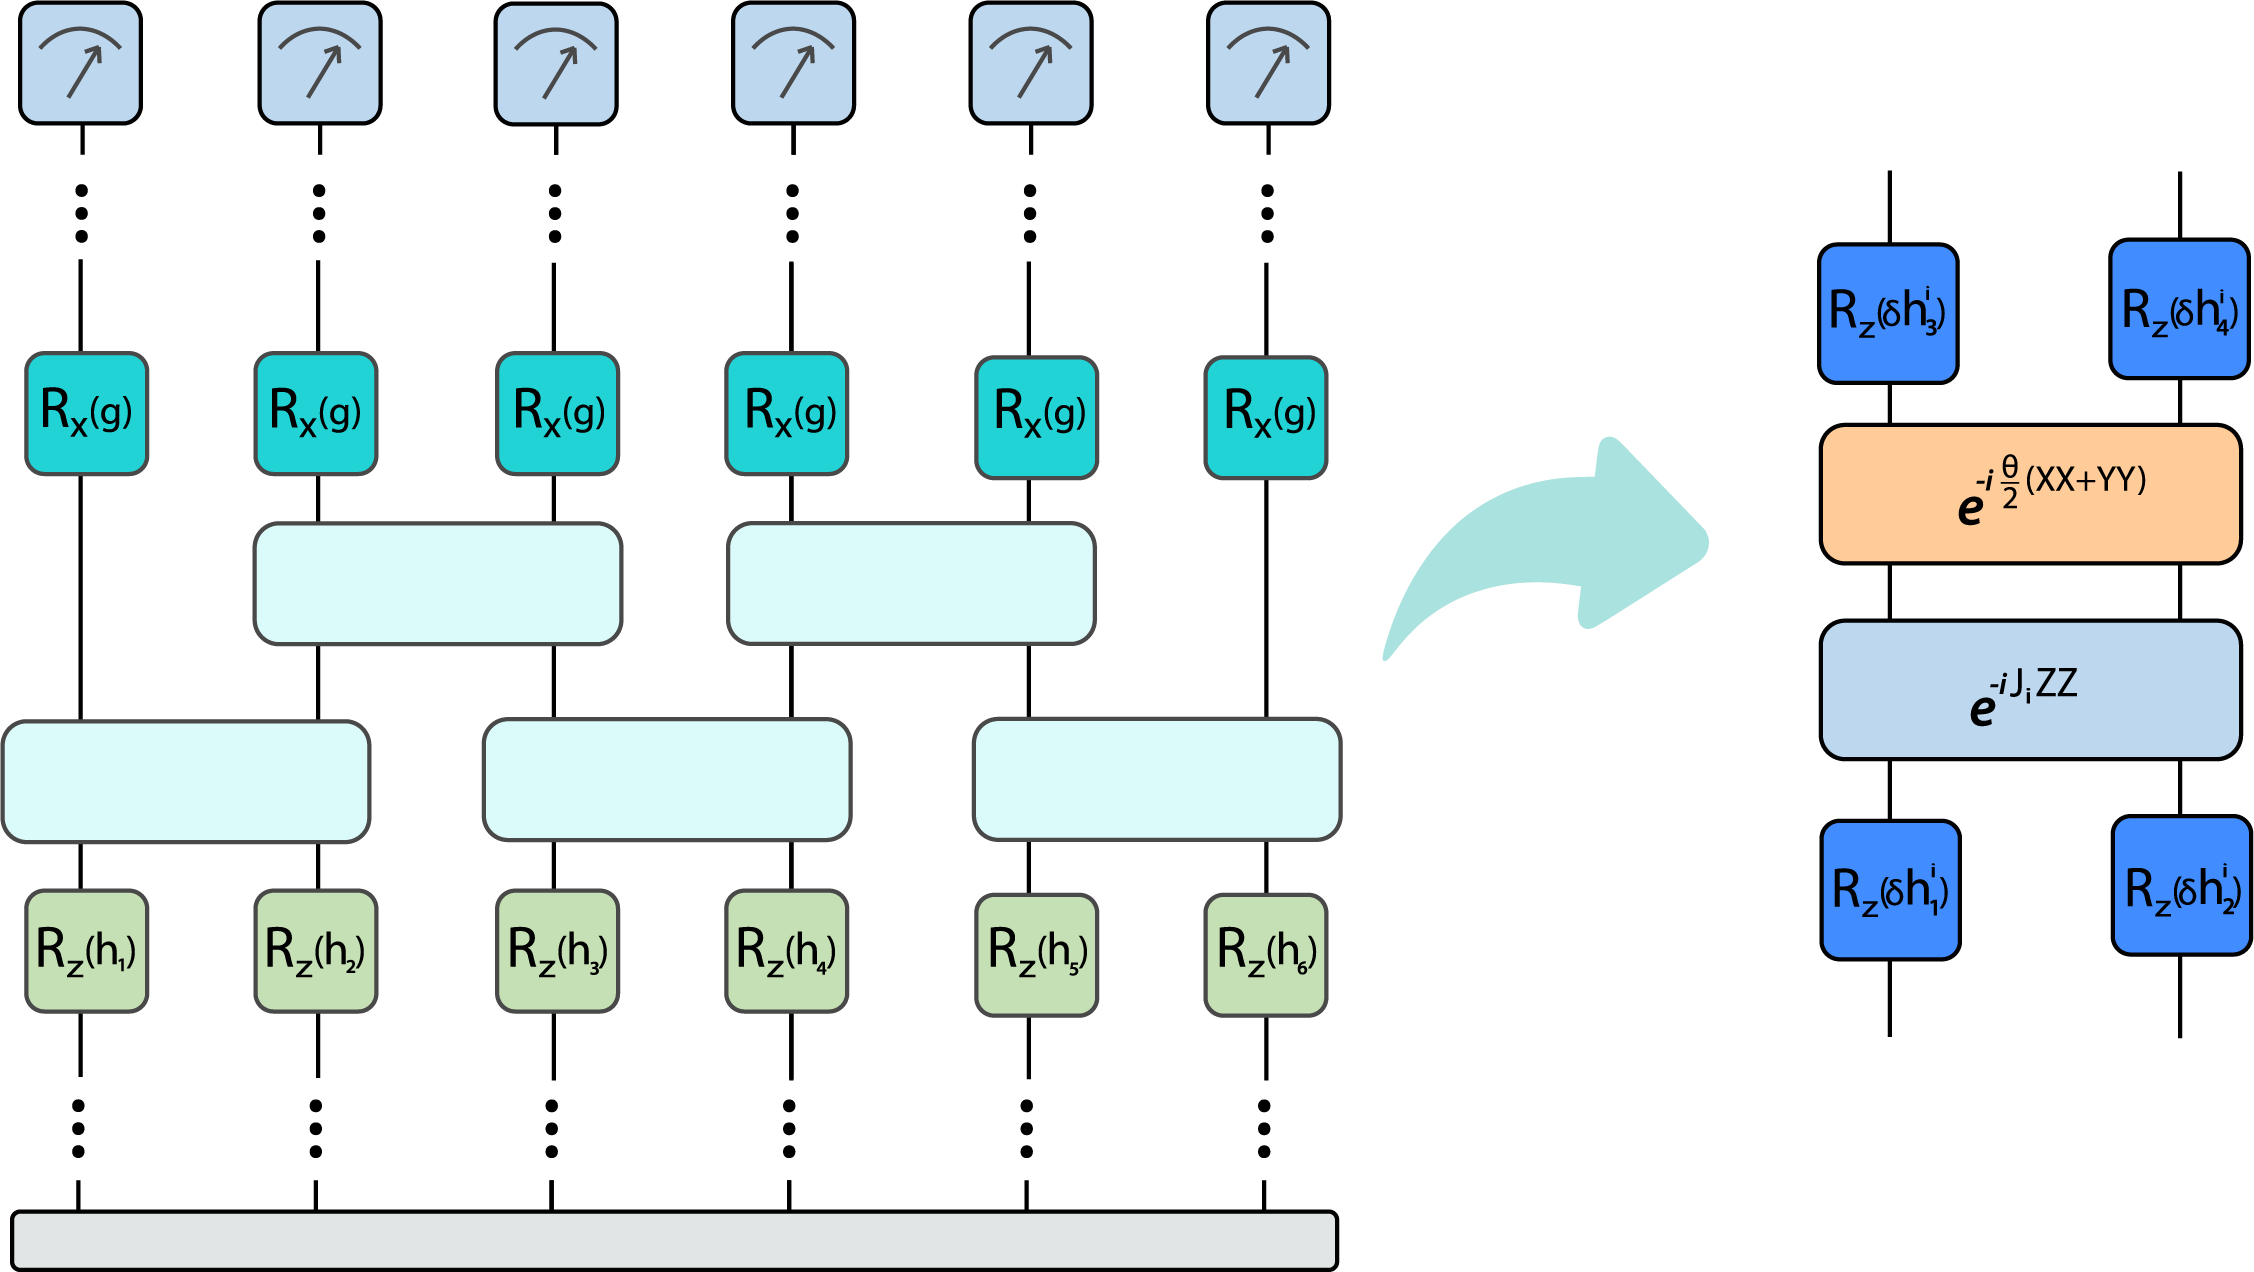
\includegraphics[width=0.9\linewidth]{./.src/images/DTC_circuit.png} 
\label{fig:subim2a}
\end{subfigure}
\begin{subfigure}{0.39\textwidth}
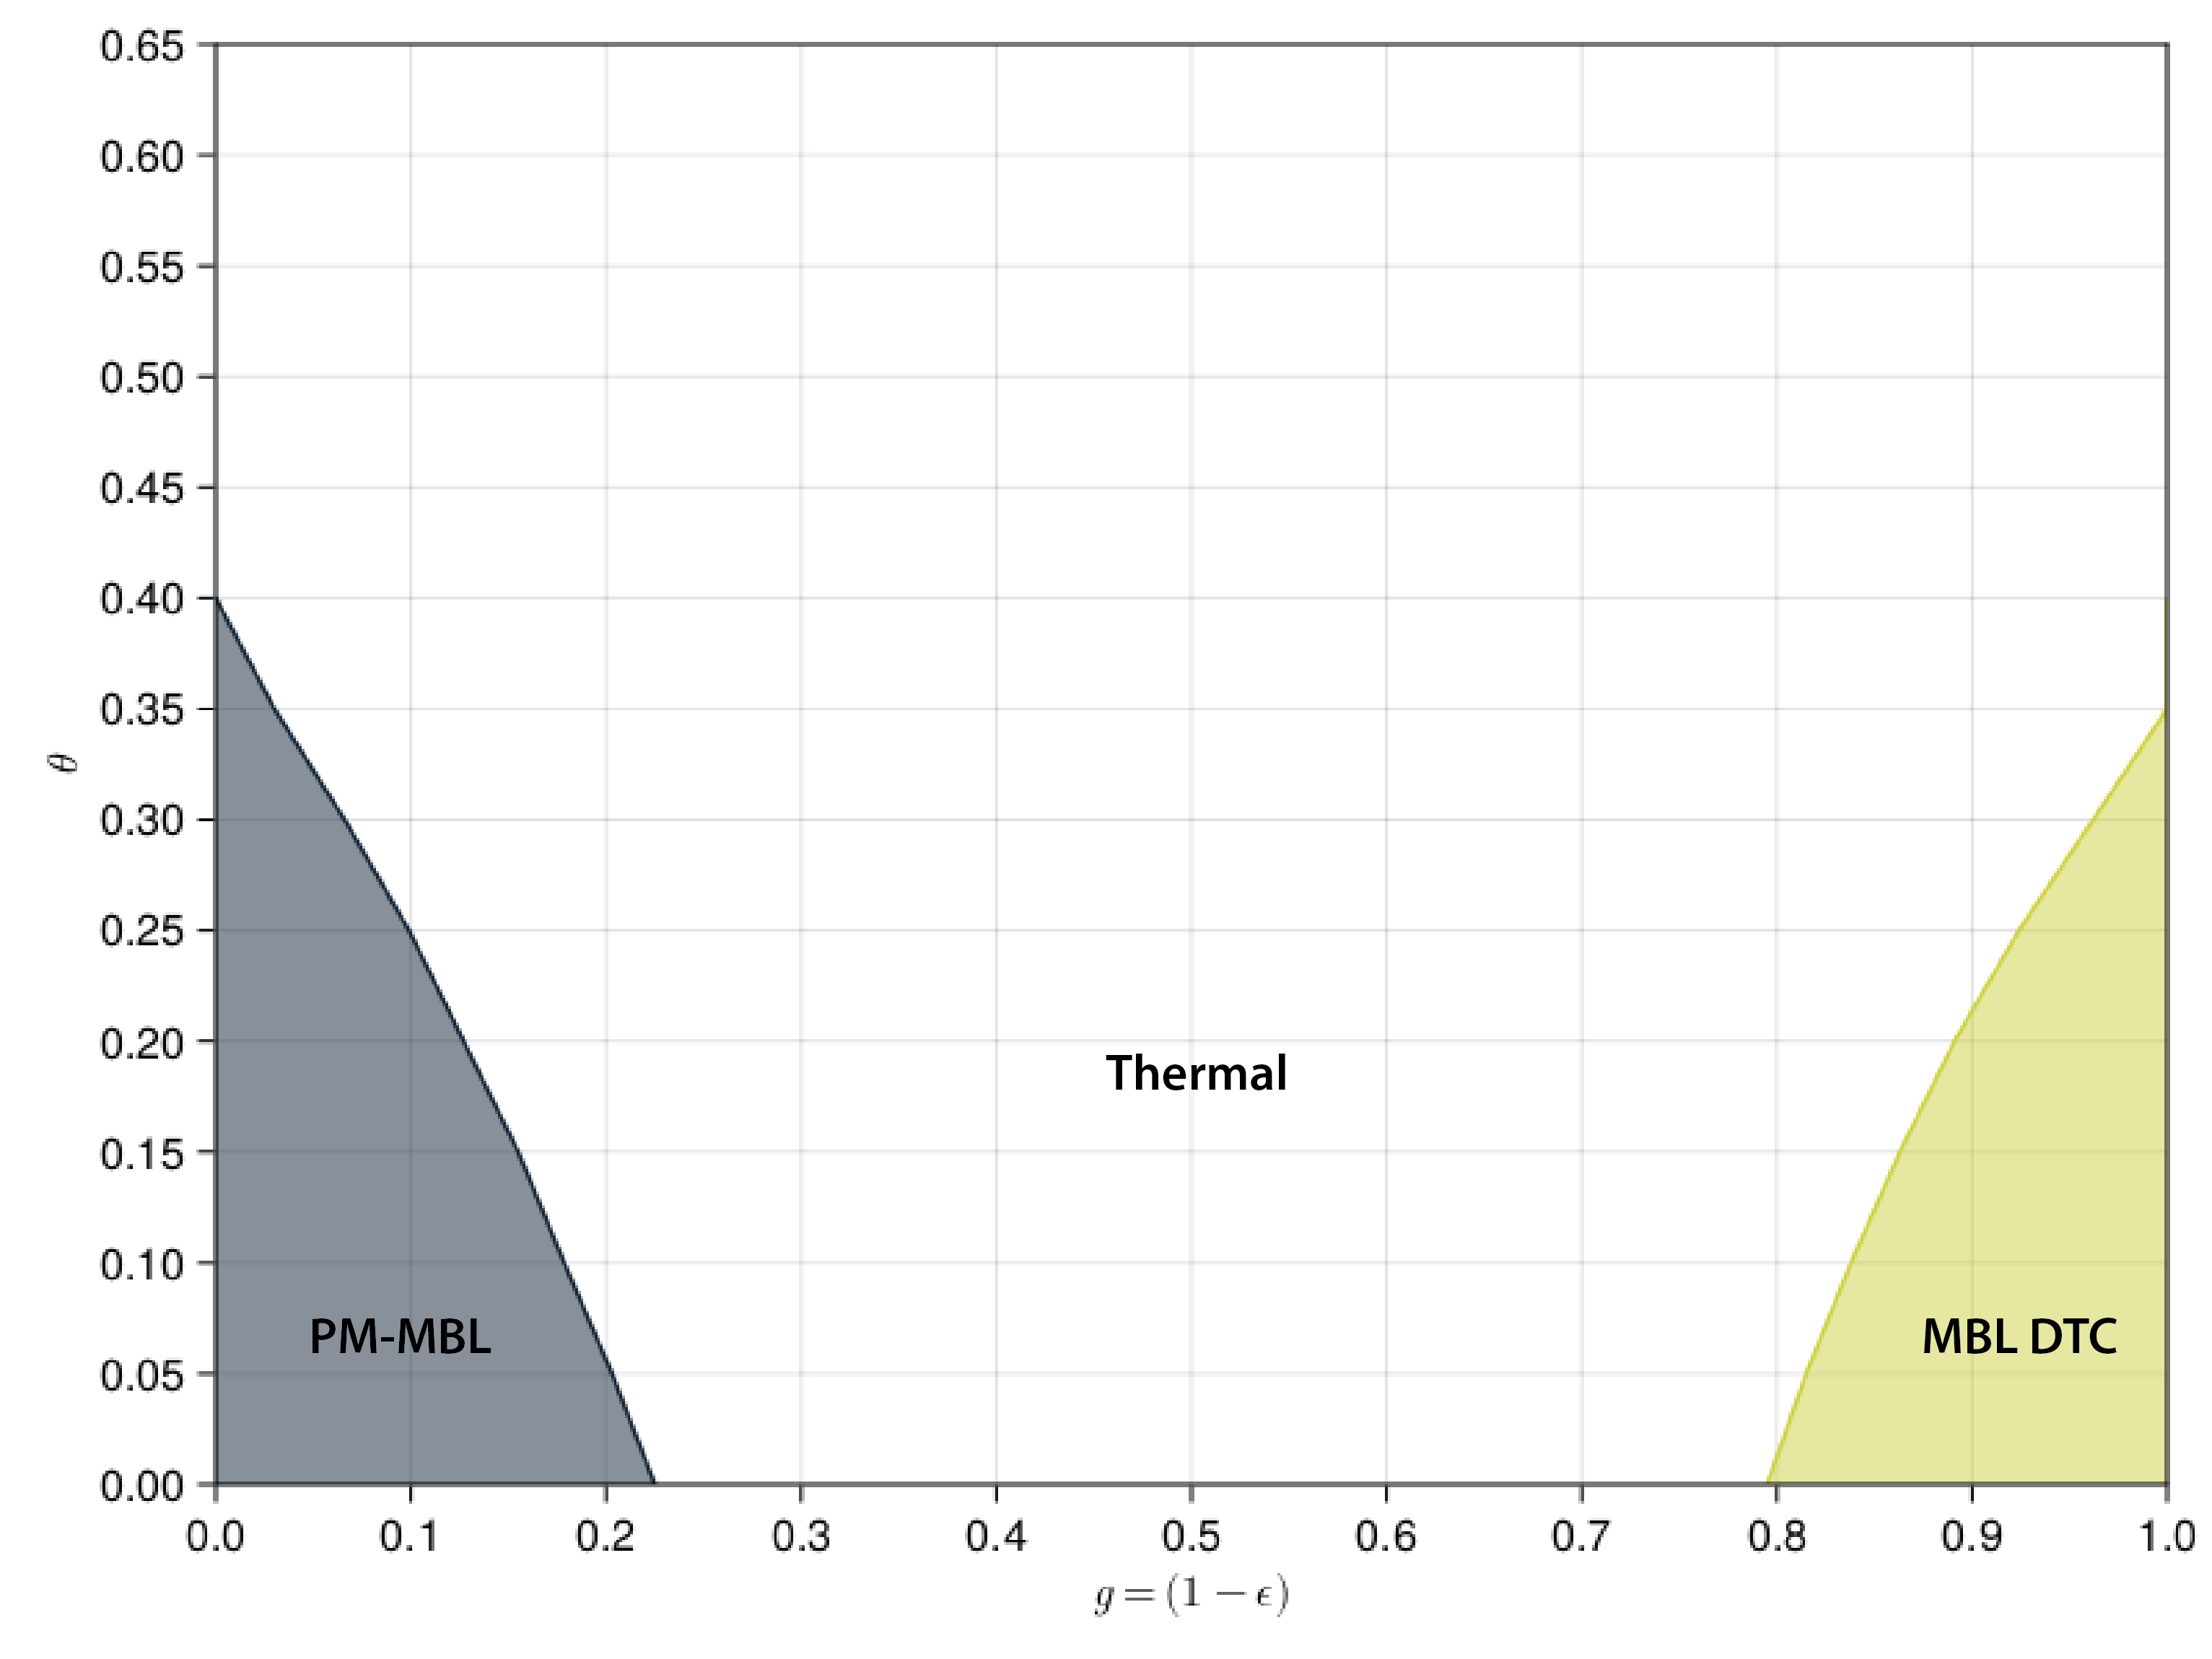
\includegraphics[width=0.9\linewidth]{./.src/images/Phase_diagram_Labeled.png} 
\label{fig:subim2a}
\end{subfigure}
\caption{Schematic representation of the circuit and the associated phase diagram. The circuit exhibit three phases. For smaller values of $\theta$ and $\epsilon$ close to 1, that is $g$ close to 0, it can support a MBL phase which is paramagnetic in nature. For small $\theta$ and $\epsilon$ close to 0, that is $g$ close to 1, it supports a DTC MBL phase with a period multiplicity of 2. In the middle region the system tend to scramble. The phase boundary was extracted from results of \cite{Khemani2021DTCinNISQ}, and was obtained from finite size scaling of the disorder averaged level spacing ratio.} 
\end{figure}

Among these parameters $J_i, h_i$ are disordered and are uniformly sampled from $[0,\frac{\pi}{2}]$ to ensure localisation and thereby to prevent the system from heating up to triviality from the kicks \cite{Khemani2015phasestructre}. In absence of interaction and with perfect kicks it is trivial to see that operators of the form $\braket{Z(0),Z(n)}$ breaks the discrete time symmetry and exhibits a period doubling. The non-triviality of the DTC as a \textit{phase} comes from the fact that this feature persists strongly even in the presence of interactions as well as with imperfect kicks (i.e $g=\frac{1}{2}=(\pi-\epsilon)$ with finite but small $\epsilon$). 

In a quantum device this is realised as a brick-wall circuit. 

%insert image of circuit

We also add further small uncertainties in the realisations of the two body gates 

\begin{equation}
    \theta=[\Bar{\theta}-\frac{\Delta\theta}{2},\Bar{\theta}+\frac{\Delta\theta}{2}]
\end{equation}

where $\Delta\theta=\frac{\pi}{50}$ and random single body $Z$ gates, $RZ(\Delta h)$, to both the legs before and after the application of the two body gates. $\Delta h=\frac{\pi}{50}$.
